\chapter{Literature Review}
This section reviews various academic sources related to the methodology proposed. It will look at the various fields of engineering as well as bio-mechanics, biomimicry and applied mathematics to form a holistic understanding of the design space. Importantly the technologies discussed will also be related to the field of robotics as many concepts transfer easily from bipedal humans to bipedal robots.

\section{Introduction}
This research project brings together various disciplines of research. By combining techniques from computer vision, sensors and data fusion we can design and develop new way of capturing human gait data. Whilst the fields of biomimicry and bio-inspired robotics are relatively new, recent advances in related fields such as artificial intelligence and robotics have invigorated the pursuit of functional humanoid robotics. 

Kaneko et al. described various components of humanoid robotics in \cite{kaneko2002design}. Herein a fundamental element of dynamics is discussed and improvements to the robots mobility outlined as the first step in the iterative design process. The same author published work \cite{kaneko2002legs} relating to a functional leg module to be used for such robotic projects. These works shows that engineers have been trying to replicate the bipedal motion of humans for some time wit relatively limited success.

If we observe some of the worlds foremost attempts at bipedal robotics such as Boston Dynamics' Atlas \cite{bdyt} and Agility Robotics' Cassie \cite{aryt} we can see that recent attempts are improving rapidly. This thesis believes that with bigger datasets of human motion in complex environments we can better design and control robotic lower limbs. 

\begin{figure}[!ht] 
\captionsetup{width=0.8\linewidth, font=small}  
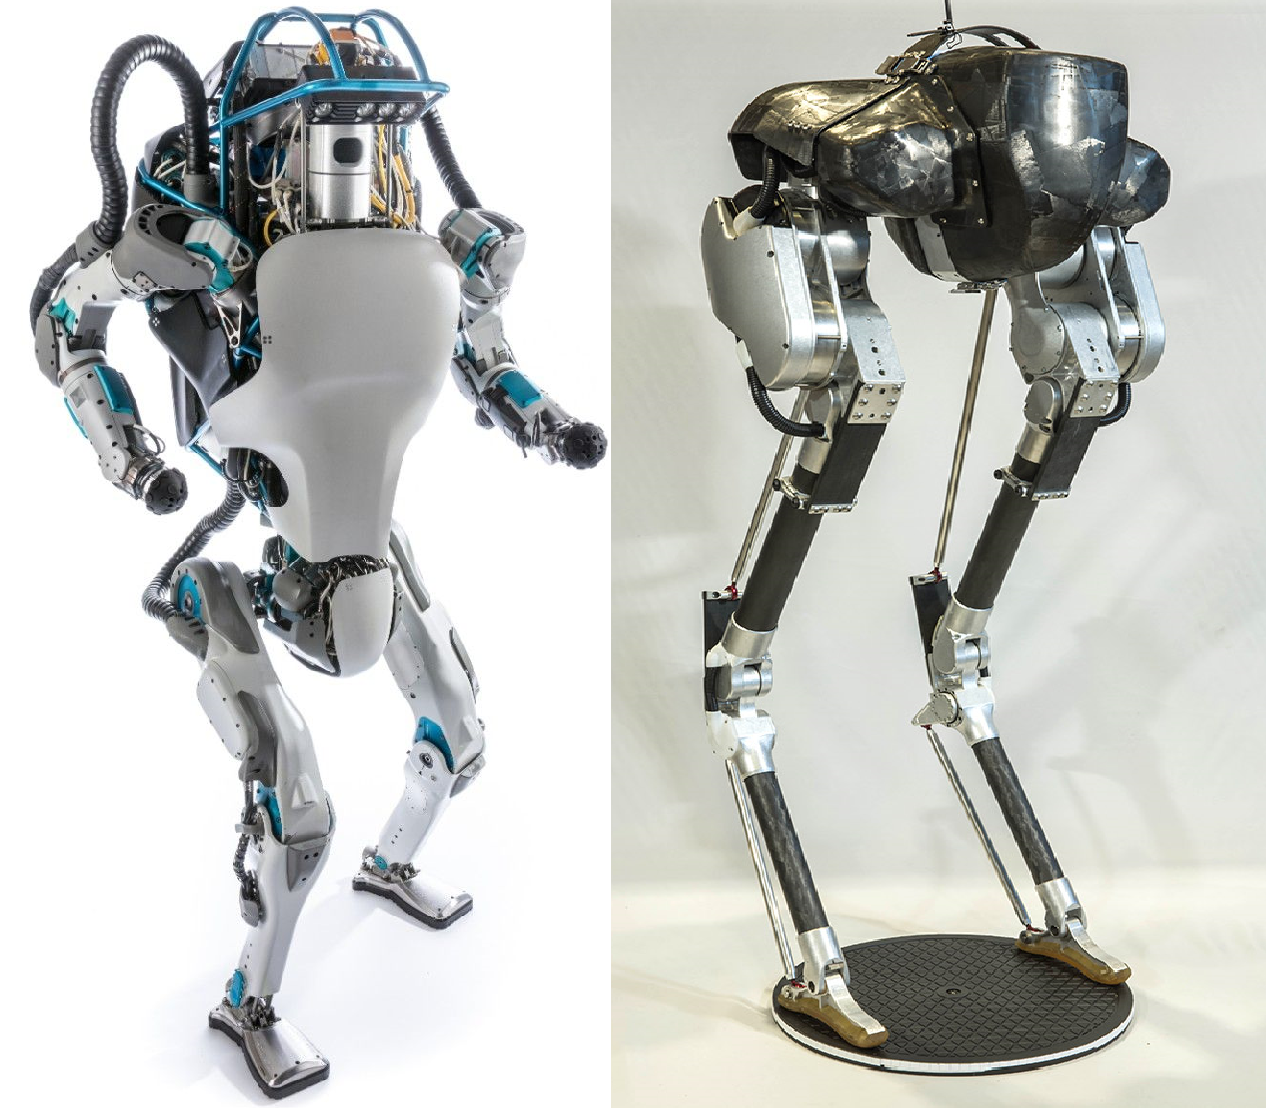
\includegraphics[width=0.8\linewidth]{figures/bipeds.png}
\caption{Pictures of modern bipedal robots Atlas (left) and Cassie (right) from \cite{bdpic} and \cite{arpic} respectively}
\label{fig:bipeds}
\end{figure}

\section{Human Motion and Gait}
The human gait is well understood and has been studied in detail as it is a fundamental part of human mobility. It is one of the first skills developed in infancy and its importance for healthy develpoment, as outlined by Adolph et al. \cite{adolph2013road}, cannot be understated. Walking and running are also critical factors in transportation and geographical movement of people and goods in developing countries where public transport is underdeveloped and private transport not within the means of the populous. Finally walking and running as exercise has proven benefits as shown in \cite{hanson2015there} (general health) and \cite{fox1999influence} (mental health). There is thus clear evidence that the human gait has earned its right as a field of study in academia.

\section{Computer Vision}
While the previous section answers "why" understanding the human gait is important, the following sections will explain fields that contribute to the question of "how" the gait is studied. The technologies and methods used to quantify it. This section titles computer vision should be interpreted within the context of this document. It will be used interchangeable with image processing as the underlying philosophies of both methodologies are algorithmic interpretation of images.

Image processing as a field was born from digital signal processing as it relates to the extraction of critical data from noisy data streams. Computer vision is the use of computational methods to achieve the same end goal. The image processing used in this thesis is basic feature detection and therefore advanced image identification task and   

\subsection{Computer Vision in Robotics}
Recent improvements to real time image processing has allowed amazing technological breakthroughs in fields closely related to robotics. One such breakthrough is the rapid improvement of self-driving cars developed by Tesla. These vehicles use vision based technologies and real time image processing to navigate complex and changing road networks. The figure below shows how a Tesla identifies different roadside artefacts.

\begin{figure}[!ht] 
\captionsetup{width=0.8\linewidth, font=small}  
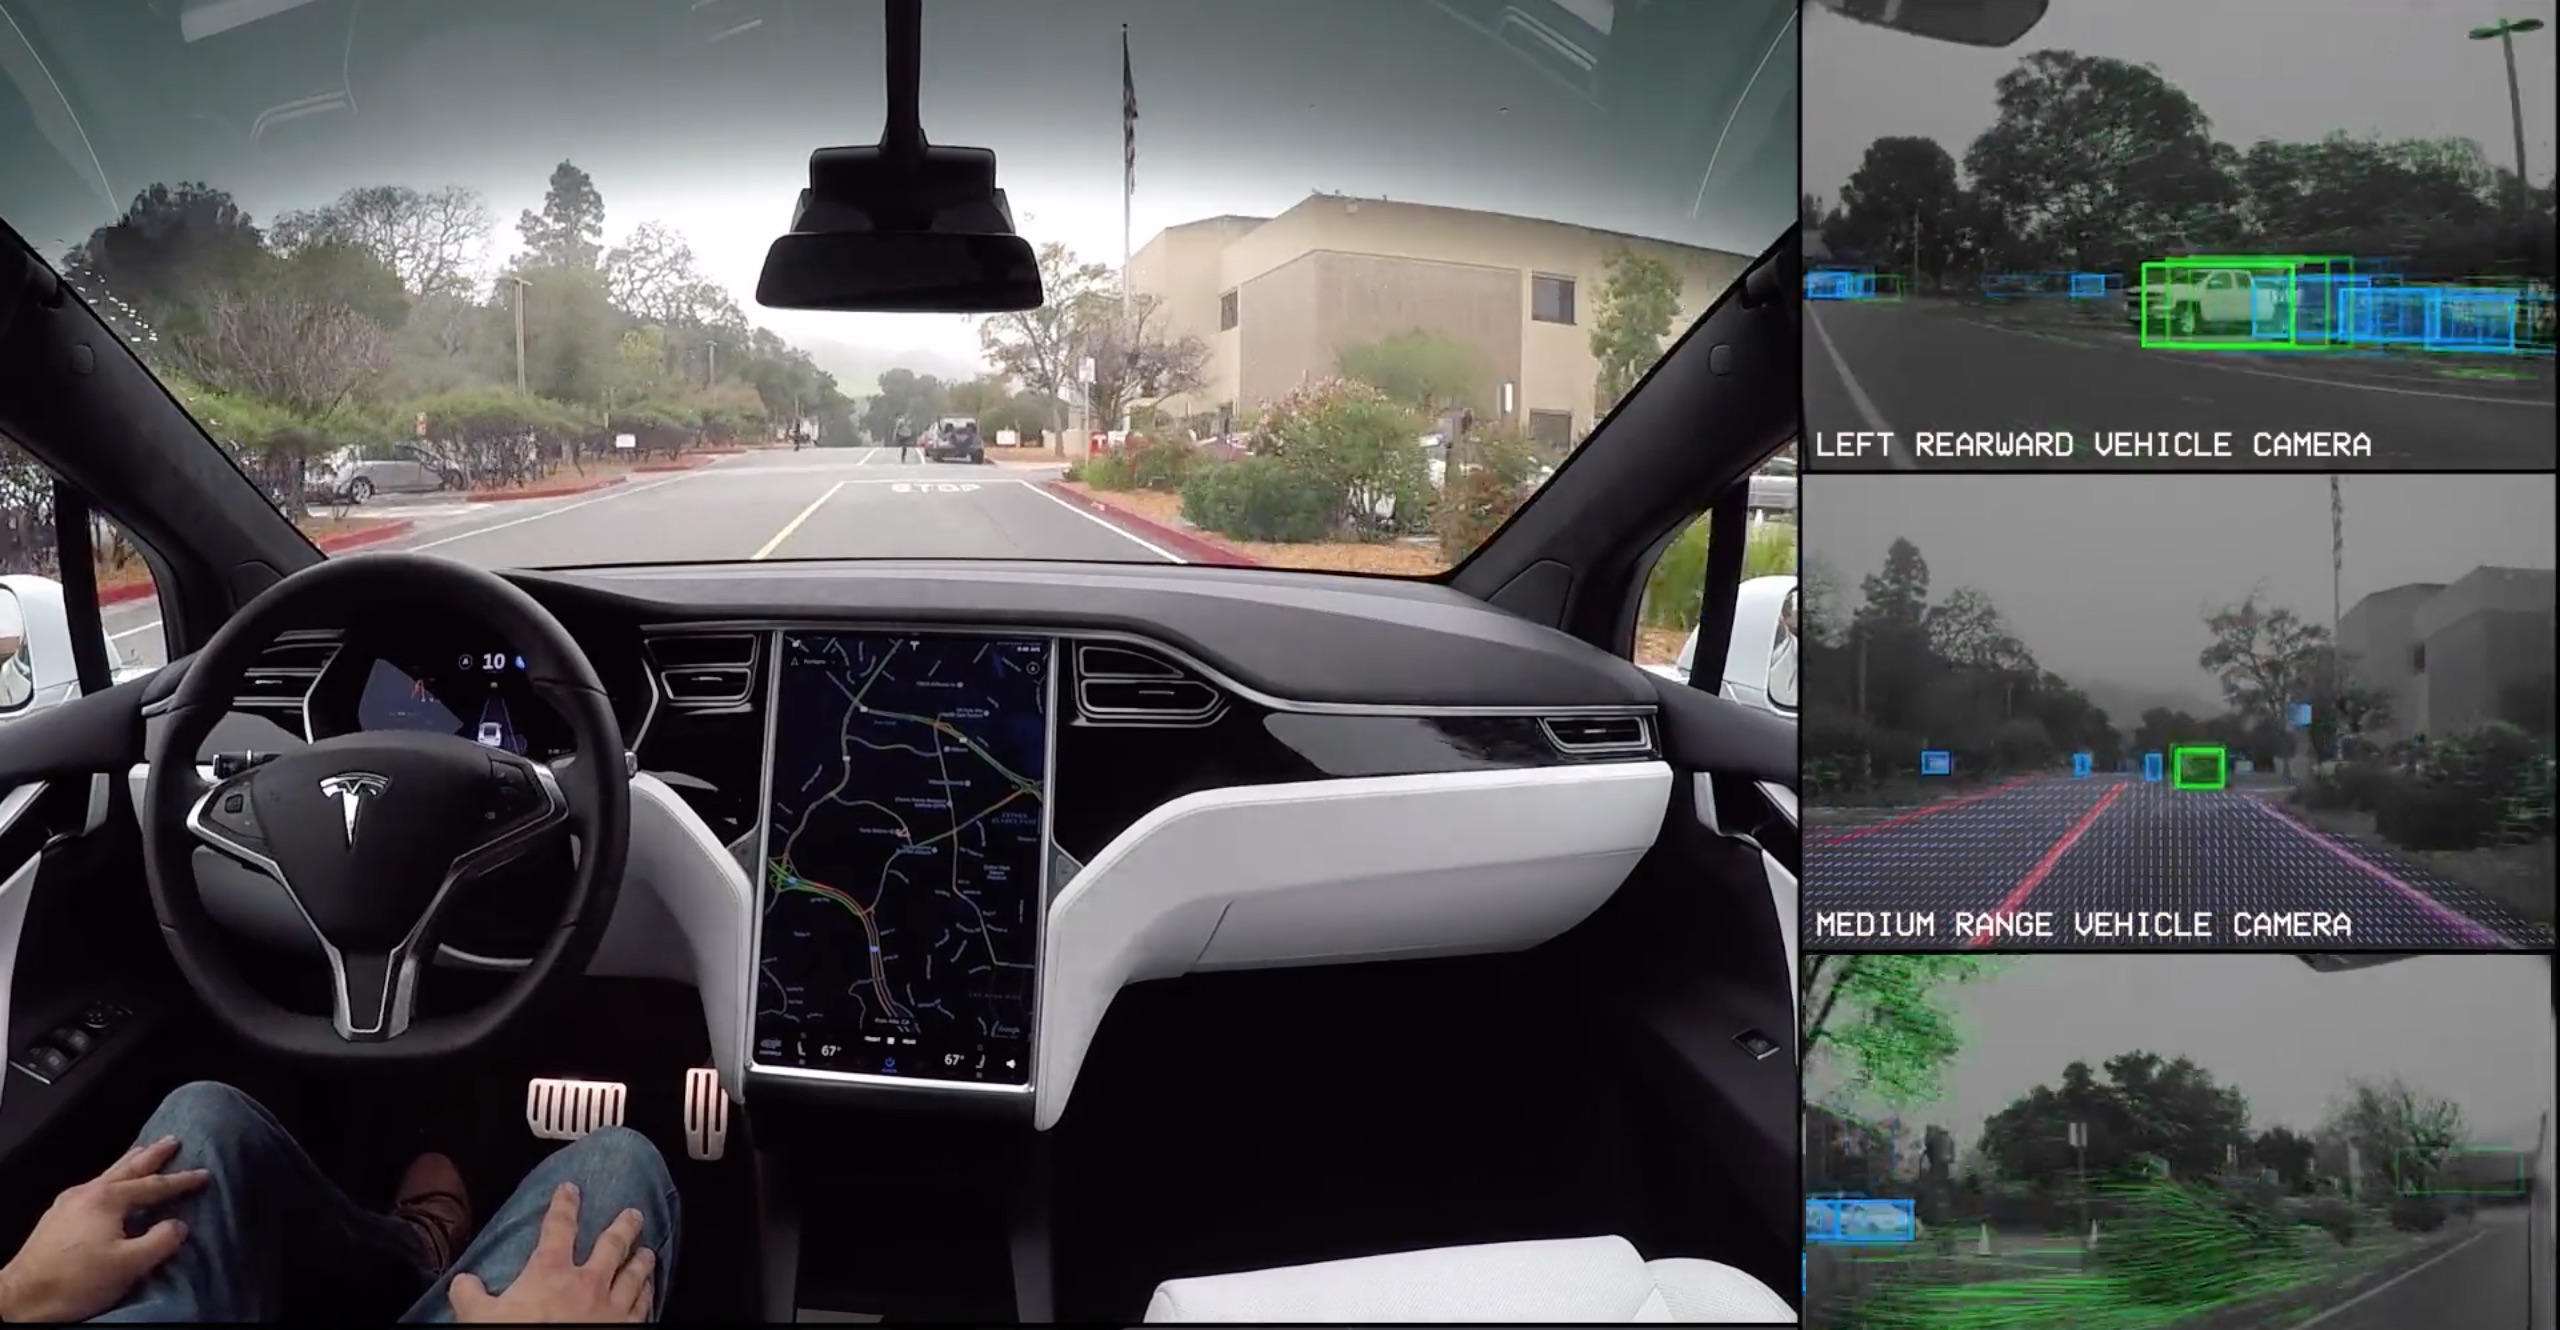
\includegraphics[width=0.8\linewidth]{figures/teslaauto.jpg}
\caption{Insight into object classification by Tesla, image from 	\cite{tesla}}
\label{fig:teslaauto}
\end{figure}

\subsection{New Perspectives from Animal Borne Cameras}
Patel et al. \cite{patel2017trackingieee} showed that using animal borne cameras and motion sensors, the tail kinematics of the cheetah (Acinonyx Jubatus) could be tracked. Patel's work was partly inspired by Kane et al. \cite{kane2014falcons} where falcon (Falco Peregrinus) borne cameras were used to better understand airborne pursuit of prey. Giving researchers a new perspective on the behaviour of animals in the natural world.

Further work completed by Pearson et al. \cite{pearson2017testing} showed that cameras mounted to dolphins (Lagenorhynchus Obscurus) could provide insight into the their movement, social and foraging strategies. Using cameras to study ocean-life has become a popular methodology in recent time due to difficulties imposed by their environment. In essence We struggle to understand flying and swimming animals due to their complex environments.

The above research has shown the unique benefits of having cameras and sensors mounted to the subject in question. 

\subsection{Human Motion Analysis Using Computer Vision}
From Chen et al.\cite{chen2013survey} using depth imagery to understand human motion we can see that this is a popular technique. Imagery has been a popular approach to interpreting human movement and gesture. Naturally this has formed a foundation of using cameras to capture human movement.

One system often used for motion capture is the Microsoft developed Kinect. \cite{gabel2012full} \cite{stone2013unobtrusive} \cite{clark2013concurrent} have shown positive results in modelling and quantifying the human gait using this technology. Interestingly all these works require controlled environments due to the nature of the technology. 

\section{Inertial Measurement Units and Sensors}
IMU's are a staple of electrical engineering as applied to dynamic systems. These sensors give us insight as to how an object is moving in space by providing data relating to orientation and acceleration of said system. These data points are created by electronically interpreting signals generated by micro-electromechanical system (MEMS). Modern smartphones have built in IMU's that are not only accurate \cite{gikas2016rigorous}, but also easy to interface with due to the open source nature of the Android operating system \cite{androidSensorLib}.  

Generally Smartphones contain the following sensors:
\begin{itemize}
\item Accelerometer
\item Gyroscope
\item Magnetometer
\item Barometer
\item Temperature
\end{itemize}

\textbf{Accelerometers} provide linear acceleration data; these accelerations may be constant (eg. gravity) or changing (eg. relative motion). In smartphones they are usually based on MEMS that use various mechanical phenomena to determine motion. 

\textbf{Gyroscopes} provide rotational data of the sensor relative to the inertial frame.  These sensors generate angular velocity data by using .

\textbf{Magnetometers} provide information relating to the macroscopic magnetic fields in a certain area. These sensors can measure the direction, strength, or relative change of fields in three different dimensions relative to the smartphone. 

\textbf{Barometers} are finely tuned atmospheric pressure sensors that can determine pressure an object is experiencing. By combining this pressure data with a well defined map of different pressure the the relative height with respect to sea-level can be calculated.

\textbf{Temperature} sensors generate local temperature data of the surrounding environment. They are important in smartphones that use lithium ion or lithium polymer batteries that can explode at high temperatures.

These sensors can be used together to better model the position, velocity and acceleration of a modern smartphone. This is easily seen when a smartphone rotates the display when held in landscape.


\subsection{Global Position System}
GPS (Global Position System) is a space based navigational system that uses satellites to determine a receivers absolute position on earth. This system was developed by the United States Air Force ion 1973 and made available for public use in the 1980s. It has since been inproved by the addition of satellites and 


\subsection{Inertial Measurement Units in Robotics}
IMUs are integral in the functioning of robotics. Up until very recently intelligent robotic systems had no sense of vision to provide feedback for their internal control systems. Instead this feedback was generated by various sensors providing information about the dynamics of these systems. \cite{kaneko2002legs} showed the importance of feedback to control bipedal robotic lower limbs. This feedback is achieved with different electronics components including gyroscopes and accelerometers; they are preferred above potentiometers since they do not mechanically intrude on the system.

\subsection{Human Motion Analysis Using Sensors}
Picerno completed and extensive review of motion sensor based data capture for human motion in \cite{picerno201725}. 

Some new methods using interesting sensors have been developed to log human motion. \cite{wang2014wearable} showed that by using highly sensitive strain sensors positioned on various joints the movement of such points of interest could be quantified. Another exotic method is the use of soft carbon nanotube capacitive sensors as in \cite{cai2013super}. These sensors are flexible and non intrusive allowing comfortable data capture.

A low cost approach in the form of a smartphone and wrist mounted sensors was used by \cite{shoaib2016complex} to show alternative methods to interpret human arms movements. Finally software developments by \cite{sun2017new} has allowed for more accurate simulations to be produced using inertial sensors. These papers are recent and shows that modern technologies and approaches to capturing motion data are being developed.


\section{Mathematical Modelling}
The binding element presented in this work is the underlying mathematics. Using various mathematical tools and methods known to robotics and bio-mechanics it is possible to transform various data types in various frames of reference to a singular model.


\subsection{Mathematical Models of the Gait}
Before exploring complex methods and tools used to analyze the human gait, it is important to select and understand the model they are derived from. Due to the large amount of existing research related to the human gait some models have been well established. These models are capable of quantifying important elements of the human gait such as gait period, dynamic joint forces and neuromuscular control. 

Some fundamental work complete by Zajac, Neptune and Winters will be discussed to better understand existing models.

In work completed by Zajac et al. \cite{zajac1990modeling} it is interesting to note the how modelling difficulties are compared to that seen in bipedal robotics. In this work he also places some important bounds on human joints. He argues that the maximum DOF (Degrees of Freedom) that any single joint can have is 6; 3 for translation and 3 for rotation. He also constrains body segments as rigid and that the internal happenings of a body segment is insignificant. 
 
In further papers published by these authors \cite{zajac2002biomechanics} and  \cite{zajac2003biomechanics} various dynamic simulations are tested against proposed methods and subject studies. These papers confirm the multi rigid segment model for studying human dynamics. Since this study is only concerned with the kinetics the assumption can be made that the model is adequate in kinematic analysis. 


\subsection{Linear Kinematics}
By using kinematics we can quantify and understand the movement of the lower limbs. Kinematics is a branch of mechanics that fully defines the motion of a point with respect to position, velocity and acceleration (be it linear, rotational or a combination). Kinematics does not however describe the forces, torques or other variables that may affect that point. This is due to a fundamental assumption in kinematics that the point is massless.	 

Kinematics can be broken up into 2 main branches: \textit{forward} and \textit{inverse}. To illustrate the matter the following diagram is that of a basic kinematic model.

\begin{figure}[!ht] 
\captionsetup{width=\linewidth, font=small}  
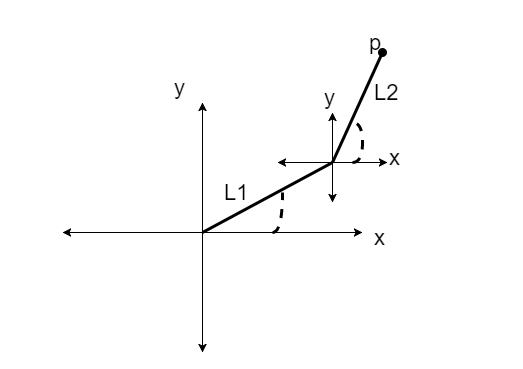
\includegraphics[width=\linewidth]{figures/kinematics.png}
\caption{Basic kinematic model to demonstrate}
\label{fig:kinematics}
\end{figure}

In this figure the position of point P is defined by 2 lengths, L1 and L2 with different lengths and angles from a set of shared axis. In forward kinematics we can find P if we know the angles and lengths of the different links in the system. The motion of point P can then be described by looking at  how the angles and lengths of the links in the system change over time.

Inverse kinematics uses knowledge of different points in the system, such as the origin and P and the lengths of the links in the system to determine the angular offsets of each length. Since these produce a set of linear equations, the more unknowns we are faced with the more possible solutions we can generate.

As discussed in the previous section a common method of modelling the human lower limbs is to use a collection of rigid beams. 


\subsection{Rotational Matrices}
There is an underlying difficulty in mathematically fusing various data sources and models; that of finding a common frame of reference. With the intent of using Lagrangian mechanics good definitions for the different frames are critical. This thesis will primarily use 2 different frames of reference. The inertial frame and the body frame.

The inertial frame (or world frame) can be defined in different ways as seen in \cite{soechting1992moving}, for the purpose of this study  the NED (North East Down) definition is used. This configuration is also known as the local tangent plain and is often used in aviation. 

Rotational matrices are mathematical objects that rotate vectors in three dimensional space. Since most engineering is constrained to the physical three dimensional world these matrices commonly rotate 3 dimensional vectors with a 3x3 sized matrix. 


\subsection{Kalman Filter and Extended Kalman Filter}
The Kalman filter is a mathematical tool used to estimate the states of a system. All measurements contain some unwanted elements of noise that produce uncertainty. Another source of uncertainty is the imprecision in the model. Simplifying assumptions disregard the minute details that when summed can have an effect on the interpretation of the data. To minimize these uncertainties it is important to filter the datasets correctly. Fortunately, estimation can be used as a form of filtering to reduce the impact of these uncertainties.    

Another powerful element of the Kalman filter is its ability to fuse data from different sources to compute a more holistic picture of the underlying system. Fusion allows us to interpret sensor data within constraints of other sensors, creating a more accurate dataset. For example we can negate the drift of an accelerometer if we have absolute positional data provided by a GPS. 

There is also an important distinction to be made between the KF and the EKF. To briefly explain this it should be understood that the Kalman filter was the original concept as developed by Rudolf E. Kálmán and he EKF the extension of said work. The KF has an inherent limitation that it can only be applied to linear systems, whereas the EKF can be applied to non-linear system operating within a certain defined range.

The KF itself can be broken down into 2 fundamental stages of operation; a prediction stage and update stage. The prediction stage takes the known current states of the system and estimates what the measurements should be for the next time interval. The measurement stage takes in current measurements and mathematically determines the states. The states of the system are user defined parameters that can often not be directly measured.

%%Systems control engineers define the cost function. Within the field of optimal control we want to control system behaviours using minimal input and with minimal error. the cost function is a mathematical representation of these extremes. 

\section{Natural Solutions for Robotic Shortcomings}
Naturally the question arises:  why would we want to better understand the dynamics of animals? A persistent problem in the field of modern robotics is that of mobility; robots struggle to navigate real world surfaces and obstacles. Work by Patel et al. \cite{patel2013rapid} shows how we can look towards nature for inspiration to solve this mobility problem. 

As demonstrated by various prototype robots built by Boston Dynamics bipedal robots are severely limited in manoeuvrability when compared to animals. This is due to the longest iterative design process known to man, evolution. Pictured below is a collection of bio-inspired robots build by Boston Dynamics.

\begin{figure}[!ht] 
\captionsetup{width=0.75\linewidth, font=small}  
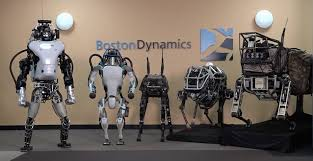
\includegraphics[width=0.75\linewidth]{figures/boston.jpg}
\caption{Different bipedal and quadroped robots created by Boston Dynamics, image from \cite{bostondynamics}}
\label{fig:boston}
\end{figure}  


\section{Conclusion}
This chapter has shown the direct parallels of technologies related to gate capture to dynamic robotic systems. With these strong parallels in mind the transferability of these systems from humans to humanoid robots is clear. In the same manner we are able to take a bio-mechanical look at the human body and treat it as a dynamics mechanical system instead of the complex bio-chemical and physiological system it really is.

This technique of abstracting systems to different domains of knowledge allows us to apply engineering methods and design to complex problem spaces. As mechanical engineers have used resistive networks to understand thermodynamics \cite{chen2015electrical} and control engineers have used mechanical models and electrical models interchangeably to apply control principles \cite{karnopp2012system}, there is power in this methodology. Fusing different methods from different fields has proven its usefulness and this work will use this approach of horizontal thinking to create its own unique methodology.

As discussed in this chapter the importance of understanding the human gait cannot be understated. The recent breakthroughs in computer vision and neural networks has reignited a field that has potential to truly change our day to day life. The ever increasing ability of sensors technology and data capture systems allow us to quantify what we have never been able to and the underlying fundamental mathematical methods never seem to fall short.

The future of humanoid robotics sits at the overlap of computer vision, IMUs and biomimicry; add to this some form of general intelligence and the world reaches a stage of automation and transformation only imagined by authors such as Asimov and Wiener. Perhaps this work could contribute to that future.

































